\subsection{Results of Topology Optimization}
A sample of ToPy's optimization process can be seen in figure \ref{fig: topyStar}. Here, a voxelized star was given as input with its end points as fixtures, and a central load normal to the star's plane. The optimization process "cuts" away unnecessary material, returning an optimally stiff structure for the specified volume fraction.

It is immediately evident that the voxel-format output of ToPy is a dead-end for designers in terms of modification and manufacturing. Thus, the next part of the workflow is fitting a smooth surface through this discrete data and arrive at a CAD format of the optimized geometry.
\enlargethispage{1cm}
\begin{figure}[H]
\centering
\begin{subfigure}[c]{.2\linewidth}
\centering
  
\includegraphics[width=.9\linewidth]{Pictures/TopOp/Star_Optimized0_Trans.png}
\end{subfigure}%
~
\begin{subfigure}[c]{.2\linewidth}
\centering
  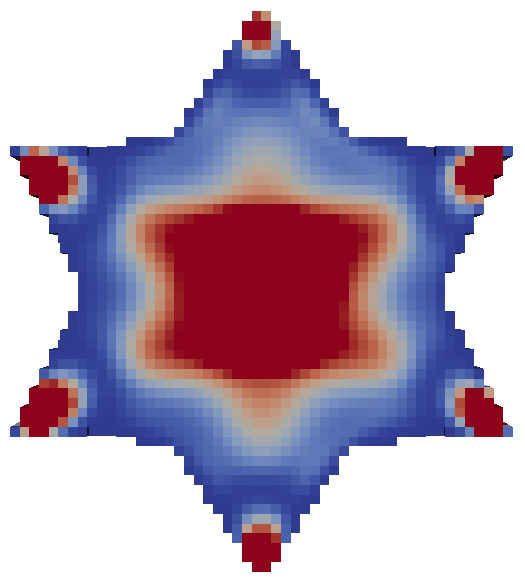
\includegraphics[width=.9\linewidth]{Pictures/TopOp/Star_Optimized2_Trans.png}
\end{subfigure}
~
\begin{subfigure}[c]{.2\linewidth}
\centering
  
\includegraphics[width=.9\linewidth]{Pictures/TopOp/Star_Optimized4_Trans.png}
\end{subfigure}
~
\begin{subfigure}[c]{.2\linewidth}
\centering
  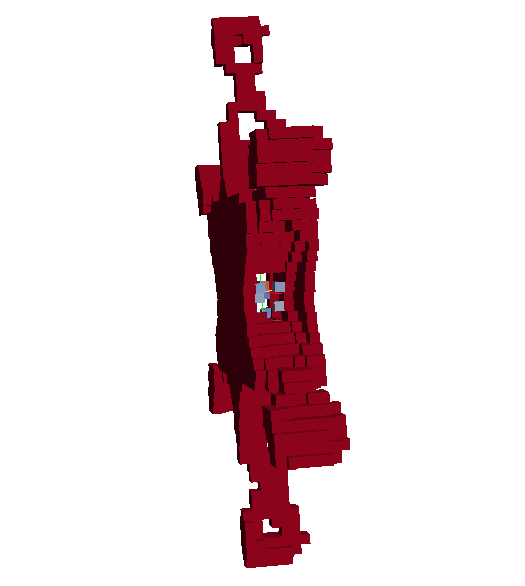
\includegraphics[width=.9\linewidth]{Pictures/TopOp/Star_Optimized5_Trans.png}
\end{subfigure}
\caption{Topology Optimization by ToPy \cite{ToPy}, with minimum compliance. \emph{From left to right}: increasing number of SIMP iterations until convergence. The star-shaped structure was given by an STL-file which was processed into input readable by ToPy, with fixtures in the corners, and a load in the middle. Throughout the SIMP iterations, one can see how material from the less dense regions (blue) is concentrated into denser regions (red) that carry the load. The last picture gives a rotated view, to illustrate how material has been eliminated even from the inside of the star. } %which volume fraction?
\label{fig: topyStar}
\end{figure}
